\documentclass[12pt, handout]{beamer}
\usetheme{Warsaw}
\usepackage{multimedia}
\usepackage{graphicx}
\usepackage{url}
\usepackage[utf8]{inputenc}

%\AtBeginSection[]
%{
%	\begin{frame}
%		\frametitle{Table of Contents}
%		\tableofcontents[currentsection]
%	\end{frame}
%}

\title{Master's thesis}
\subtitle{Simulation of complex actuators}
\author{Hubert Woszczyk}
\institute{Univerity of Liège}
\date{Academic year 2015-2016}

\begin{document}
	
\frame{\titlepage}

\section{Introduction}
\frame{\frametitle{Context \& Motivation}
	\centering
	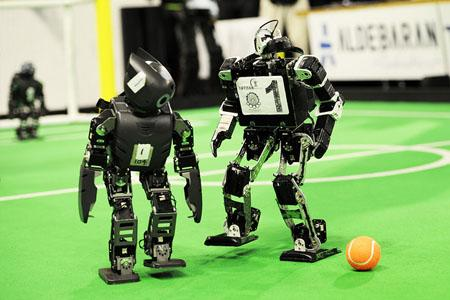
\includegraphics[width=0.7\textwidth]{images/intro_roboSoccer}
}

\frame{\frametitle{Problem statement}
	Required simulator features:
	\begin{itemize}
		\item realistic rigid bodies physics simulation
		\item constraints
		\item the model of the robot should be able to interpret the same instructions that the real robot will
	\end{itemize}
}

\section{Software solutions}
\frame{\frametitle{Software choices}
	\centering
	\includegraphics[width=\textwidth]{images/overview}
}


\section{Physics simulation}
\frame{\frametitle{Modelling (1/2)}
	\begin{center}
		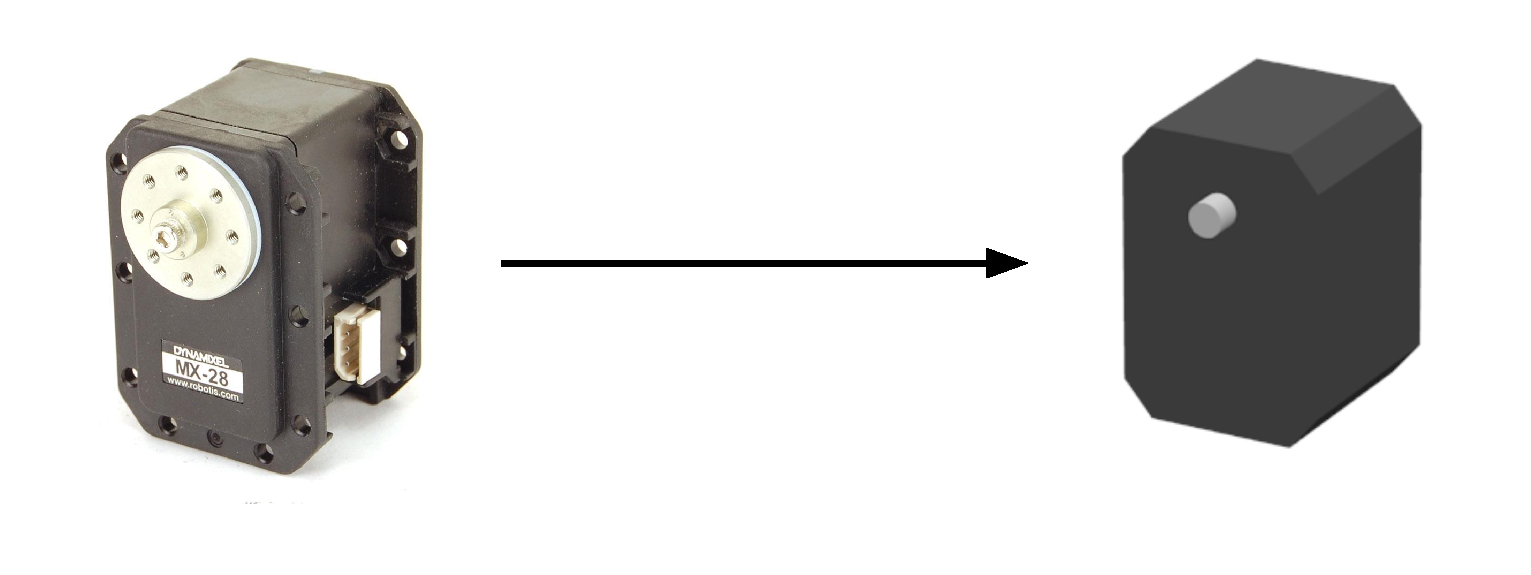
\includegraphics[width=0.6\textwidth]{images/modelling}\\
	\end{center}
	Problems : \begin{itemize}
		\item mass \& inertia
		\item volume
		\item function
		\item constraints
	\end{itemize}
}

\frame{\frametitle{Modelling (2/2)}
	\begin{columns}[T] % align columns
		\begin{column}{.48\textwidth}
			Blender :\begin{itemize}
				\item volume
				\end{itemize}
		\end{column}%
		\hfill%
		\begin{column}{.48\textwidth}
			V-Rep : \begin{itemize}
				\item mass
				\item inertia
				\item function
				\item constraints
			\end{itemize}
		\end{column}%
	\end{columns}
}

\section{Control}
\frame{\frametitle{Control (1/2)}
	\begin{center}
	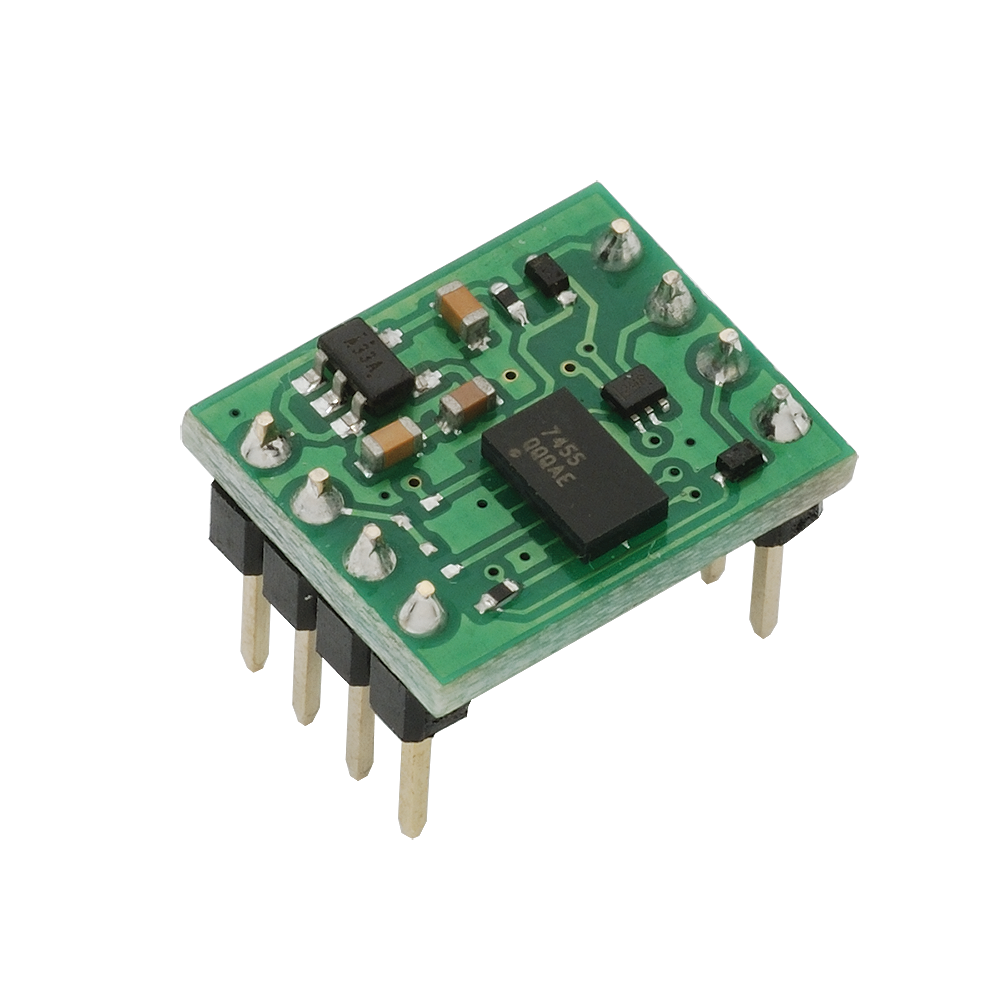
\includegraphics[width=0.3\textwidth]{images/accel}
	\end{center}
	Problems : \begin{itemize}
		\item same orders as real robot
		\item retrieve state of simulation
	\end{itemize}
}

\frame{\frametitle{Control (2/2)}
	Solutions : \begin{itemize}
		\item remote control through TCP socket
		\item synchronous operation
		\item scripts
	\end{itemize}
}

\section{Applications}
\frame{\frametitle{Applications (1/2)}
\centering
\movie[label=show3,width=0.8\textwidth, poster]{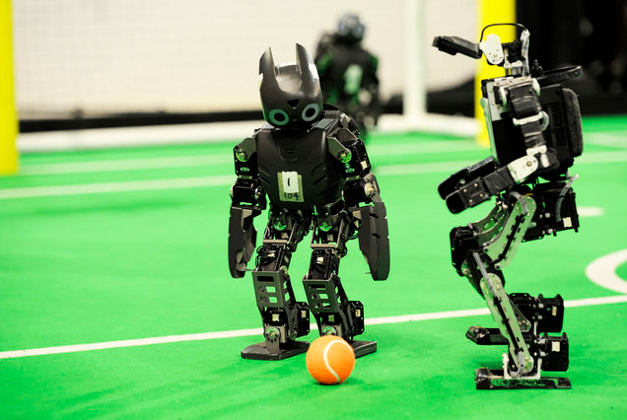
\includegraphics[width=0.8\textwidth]{images/intro_ks}}{prone.avi}
}

\frame{\frametitle{Applications (2/2)}
\centering
\movie[label=show3,width=0.8\textwidth, poster]{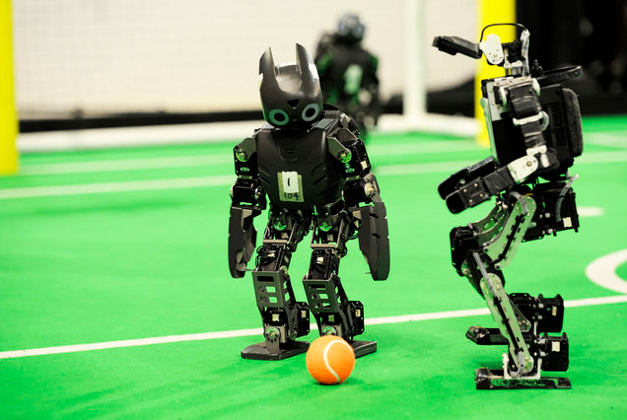
\includegraphics[width=0.8\textwidth]{images/intro_ks}}{prone.avi}
}

\frame{\frametitle{Conclusion}
	\centering
	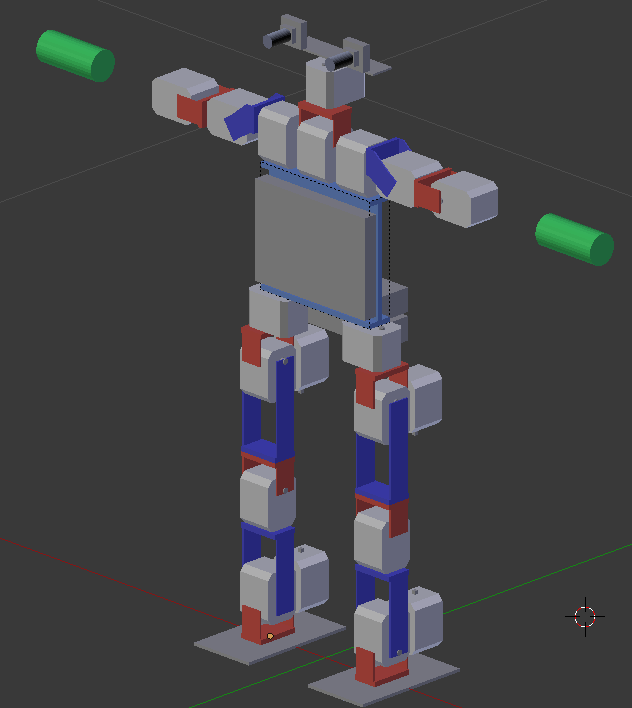
\includegraphics[width=0.5\textwidth]{images/robot_ortho}
}

\end{document}
